\documentclass[../main/main.tex]{subfiles}
\begin{document}

%%%%%%%%%%%%%%%%%%%%%%%
%%%%%%%% LECTURE 11 %%%%%%%%
%%%%%%%%%%%%%%%%%%%%%%%

\chapter{Quantum solitons}

\section{Introduction to topological objects}

The first appearance of a classical \emph{soliton} was in a report by J. Scott Russel in 1842, he was in a boat in a channel and noticed ``a solitary elevation, a rounded, smooth and well-defined heap of water which continued in course along the channel apparently without change of form (i.e. without dispersion/dissipation) or diminution of speed (i.e. constant velocity). 

The term ``soliton'' (which comes from ``solitary wave'') was much later introduced to characterize solutions of wave equations that do not dispense and preserve their form during the propagation. Hence in a sense a classical solution behaves as a particle in spite of being a wave. 

The staticity of these ``wave'' solitons is due to some conservation law. If this conservation law is of topological origin (i.e. the conserved quantity is not related to the (first) Noether theorem and the conservation holds without using all the equations of motion\footnote{For instance, the conservation of the EM current $J_\nu=\partial^\mu F_{\mu\nu}$ does not follow from the equation of motion $\der{p^\mu}{t}=F^{\mu\nu}u_\nu$, but is just a consequence of the antisymmetry of $F_{\mu\nu}$: $\partial^\nu J_\nu=\partial^\mu\partial^\nu F_{\mu\nu}=\partial^{\{\mu}\partial^{\nu\}}F_{[\mu\nu]}=0$.}) these solitons are called \emph{topological}. 

The original concept of topologically protected ``wave'' solitons has been later extended, in particular by high-energy physicists, and today we define a classical topological soliton as a topologically stable, finite energy solution of the Hamiltonian equations of motion of a classical field theory. 

Since already classically solutions behaves as particles, one can naturally expect, correctly, that their quantized version provides a quantum particle, but as we will see later it is a peculiar one. 

\subsection{Spontaneously broken symmetry}

\cite[Chapter C.1]{Strocchi_1985}, \cite{Strocchi:2012}\\

Before entering in the discussion of solitons, a brief formal discussion of the spontaneously broken symmetry (SSB) phenomenon is required. 

We already know that the \emph{observables} of a system are the quantities of the physical system that we can measure and the algebra that they generate is called the \emph{observable algebra} $\obsalg$. The \emph{states} contain the information on the system, if the information is maximal they are called \emph{pure}, if it is not maximal are said \emph{mixed}. 

By definition pure states can be obtained one from the other by operations physically performed on the system (including limiting procedure, such as the infinite volume limit or the thermodynamic limit, but excluding transformations which require to cross would-be states of infinite ). Both in the classical and quantum settings the mixed states can be viewed as complex combinations of pure states and a state is pure if it cannot be written as convex combination of the pure states. 
For equilibrium states at finite temperature by analogy we introduce the concept of \emph{pure phase}: an equilibrium state is a pure phase if it cannot be written as a convex combination of other equilibrium states.

\skipline

For instance consider the Ising model: take a finite lattice of volume $V$, where to each cell $i$ is associated a classical spin $\sigma_i$ with possible values $\pm1$. Suppose that we imposed vanishing boundary conditions, i.e. outside the volume we do not have any spin (the system is confined), and try to take the infinite volume limit. For spatial dimension $d=2$ and temperature $T<T_c$ where $T_c$ is the \emph{critical temperature} the system has two possible ground states: for the first one $\langle\sigma_i\rangle>0$ for all the cells, for the second one $\langle\sigma_i\rangle<0$. Obviously, the equilibrium state for the system in such condition is described by $\langle\sigma_i\rangle =0$ for all the possible cells, and it is not a pure phase as it can be described as a convex combination of the two ground states, which in turn are (unstable) equilibrium states. 

\skipline

We can now distinguish different kinds of symmetries. An \emph{algebraic symmetry} is an invertible algebra homomorphism $\obsalg\to\obsalg$ (i.e. a map preserving the algebraic relations, e.g.  equations of motion are preserved in form and also (in quantum setting) the commutation relations between observables). A \emph{physical symmetry} is an algebraic symmetry together with an invertible map $\purstate\to\purstate$, where $\purstate$ is the space of pure states, which preserves the expectation values:
\begin{eq}
	\begin{aligned} 
		\alpha:\obsalg&\longrightarrow\obsalg\\
		A&\longmapsto A'
	\end{aligned}
	\qquad\text{and}\qquad
	\begin{aligned}
		\tilde \alpha:\purstate&\longrightarrow\purstate\\
		\Sigma&\longmapsto\Sigma'
	\end{aligned}
\end{eq}
such that
\begin{eq}
	\langle A\rangle_\Sigma=\langle A'\rangle_{\Sigma'}
\end{eq}
A \emph{dynamical symmetry} is either an algebraic or a physical symmetry leaving the Hamiltonian invariant
\begin{eq}
	H\longmapsto H'=H
\end{eq}

A dynamical symmetry is said \emph{spontaneously broken} if it cannot be realized as a physical symmetry, i.e. is an algebraic symmetry leaving $H$ invariant but it does no exists a map in the space of pure states of the system preserving the expectation values. 

\skipline

Naively it seems impossible to define a spontaneously broken symmetry, as for each map $\alpha:\obsalg\to\obsalg$ always exists a map $\tilde\alpha:\purstate\to\purstate$ defined by
\begin{eq}
	\langle \alpha^{-1}(A)\rangle_\Sigma=\langle A\rangle_{\tilde\alpha(\Sigma)}
\end{eq}
which clearly implies
\begin{eq}
	\langle A\rangle_\Sigma=\langle\alpha(A)\rangle_{\tilde\alpha(\Sigma)}=\langle A'\rangle_{\Sigma'}
\end{eq}
What goes wrong is that such map $\tilde\alpha:\Sigma\mapsto\Sigma'$ in principle may send the space $\purstate$ not in itself, i.e. in principle $\tilde\alpha(\Sigma)\not\in\purstate$, but in another space of states not realizable by means of physical operations on the system starting from the initial states in $\purstate$.

\skipline

Take for instance the Heisenberg model of a ferromagnet in three dimension, where the spin is classically described by a unit vector in a lattice. Let's then consider the thermodynamic limit. It is well known that such system has a critical temperature $T_c$, such that for $T<T_c$ the ground states have an expectation value $\langle\vec s_i\rangle\neq0$. For $T=0$ all the spin are aligned in the same direction. The Hamiltonian for this system is 
\begin{eq}
	H=J\sum_{\langle i,j\rangle}(\vec s_i-\vec s_j)^2
\end{eq} 
which is clearly invariant under rotations. Consider two ground states at $T=0$ which differs for the orientation of the spins, and let's see if these can be related by some allowed transformation or not, if not we would have a spontaneous symmetry breaking. We are allowed to do only physical allowed (in particular, local) transformations, at least by some limiting procedure. Nevertheless we already took the thermodynamic limit, therefore we are not allowed to move all the spins (including those at infinity) at the same time with a single transformation. We are forced to use some limiting procedure, for instance we can consider neighbourhoods of circles of radius $R$ and smoothly rotate the spins in these regions, while we increase $R$ from 0 to $\infty$. But as $R$ approaches $\infty$ there are infinitely many spins rotated simultaneously, hence due to the non trivial interacting energy between spins, one can expect that such procedure requires an infinite amount of energy. If the explicit computation of the energy actually give us an infinite energy cost, then spontaneous symmetry breaking occured. 

Notice that in general one cannot guess whether we have SSB or not, a computation of the energy (or some other relevant physical quantity) is needed. 

\skipline

Unfortunately sometimes one refers to SSB in the case in which the Hamiltonian is invariant under a symmetry $\alpha$, but each of its pure equilibrium states are not invariant under $\tilde\alpha$, hence restricting the non-invariance to equilibrium states. 

For field theories are basically equivalent from the practical point of view but for systems with finite degrees of freedom they are not. For instance consider a horizontal place where gravitational force applies in the vertical direction, and put a point particle at rest a point, then certainly this describes an equilibrium state. The Hamiltonian is invariant under horizontal space translations, nevertheless the equilibrium state is not, hence according to the latter definition the symmetry is spontaneously broken. On the other side, certainly this is not a SSB according to the first definition, because we can easily move to another equilibrium state by some physically allowed translation, since all the intermediate states are pure states of the system. 

\section{Kinks}

\cite[Chapter 2]{Shifman:2012}, \cite{Gousheh_2012}, \cite[Chapters 2,5,8]{Rajaraman:1982}\\

The fist (topological) soliton that we consider is the \emph{kink} in $\phi^4_2$, i.e. the relativistic $\phi^4$ theory in 1+1 dimensions in the spontaneously broken phase. 

\subsection{Classical treatment}

The classical Hamiltonian we consider is on the real line $\R$, labelled by $x$, and if the system is described by a real scalar field $\phi(x,t)$ with conjugated momentum $\pi(x,t)$ (the dependence on time of the fields is understood) it reads
\begin{eq}\label{eq:ham-kink}
	H=\int\de x\,\ham\big(\pi,\phi\big)=\int\de x\,\left[\half\pi^2+\half\left(\der{\phi} x\right)^2+\frac{g^2}4\big(\phi^2-v^2\big)^2\right]
\end{eq}
with $v,g\in\R$. This potential is the field analogue of the double well with potential $\frac{g^2}4(x^2-v^2)^2$.
The equations of motion in Hamiltonian formalism are
\begin{eq}
	\dphi&=\fder{H}{\pi}=\pder{\ham}{\pi}=\pi\\
	\dpi&=\fder{H}{\phi}=\pder{\ham}{\phi}=-\dpder{}{x}\phi+g^2\big(\phi^2-v^2\big)\phi
\end{eq}
where for the second equation we used an appropriate integration by parts in $H$. 
Equilibrium states are given by the equilibrium condition $\dphi=\dpi=0$, which implies (for each $x\in\R$)
\begin{eq}
	\pi=0
	\tand
	\dpder{}{x}\phi=g^2\big(\phi^2-v^2\big)\phi
\end{eq}
Clearly, from the structure of the Hamiltonian, finite energy solutions must satisfy 
\begin{eq}\label{eq:kink-boundary-conditi}
	\pi\to0
	\tand
	\phi\to\pm v
	\tfor
	x\to\pm\infty
\end{eq}
as otherwise $H$ is divergent. Indeed all the terms inside $H$ are strictly positive, hence both the term depending on $\pi$ and the term depending on $\phi$ should vanish identically at infinite. The absolute minima of $H$ are given by the two configurations
\begin{eq}
	\phi_+^0=+v \tcomma \pi^0=0
	\tand
	\phi_-^0=-v \tcomma \pi^0=0
\end{eq}
In such cases $H$ vanishes, hence both these solutions are called \emph{vacuum}. The expectation values of the field at the minima are
\begin{eq}
	\langle\phi\rangle_{\phi_\pm^0,\pi^0}=\pm v
\end{eq}

\skipline

The Hamiltonian is invariant under the symmetry $\alpha$
\begin{eq}\label{eq:symm_kink}
	\phi\mapsto-\phi
	\tcomma
	\pi\mapsto-\pi
\end{eq}
We see that in order to satisfy
\begin{eq}
	\langle\phi\rangle_\Sigma=\langle\alpha(\phi)\rangle_{\tilde\alpha(\Sigma)}
\end{eq}
for $\Sigma=(\phi^0_\pm,\pi^0)$ we should have 
\begin{eq}
	\pm v=\langle-\phi\rangle_{\tilde\alpha(\phi^0_\pm, \pi^0)}
\end{eq}
which is satisfied for $\tilde\alpha(\phi^0_\pm,\pi^0)=(\phi^0_\mp,\pi^0)$.
However it is impossible to reach continuously $\phi_-^0$ from $\phi_+^0$ and vice versa, since the set of boundary conditions at infinity, $\{+v,-v\}$, is not connected and to reach one minimum from the other with (the limit of) a local transformation we need to cross infinite energy states. Therefore symmetry eq.~\eqref{eq:symm_kink} is spontaneously broken, and the two minima that we found lives in disjoint space of states related by a parity transformation.

\subsubsection{First-order equation}

However there are two local minima in the space of finite-energy solutions: we can find them with the following trick. For $\pi=\dphi=0$ the equation of motion reduces to
\begin{eq}\label{eq:eom-kink}
	\der{^2}{x^2}\phi=\frac{g^2}4(\phi^2-v^2)\phi
\end{eq}
where now $\phi$ depends only on $x$. If we think about $x$ as a time coordinate and $\phi$ as the position $q$  of a particle, then eq.~\eqref{eq:eom-kink} become a Newton equation with potential $V(q)=\frac{g^2}4(q^2-v^2)^2$. Due to energy conservation we get
\begin{eq}
	\half\dot q^2-\frac{g^2}4(q^2-v^2)^2=\tconst=0
\end{eq}
where the vanishing of the energy is due to the boundary condition eq.~\eqref{eq:kink-boundary-conditi}. Hence we can solve the previous differential equation:
\begin{eq}
	\der qt=\pm\frac g{\sqrt2}(q^2-v^2)
\end{eq}
i.e.
\begin{eq}
	\der\phi x=\pm\frac g{\sqrt2}(\phi^2-v^2)
\end{eq}
These are standard first order equations trivially solved by 
\begin{eq}
	\int\de x=\mp\frac{\sqrt2}{g}\int\frac{\de\phi}{\phi^2-v^2}
\end{eq}
which have solutions
\begin{eq}
	x=\pm\frac{\sqrt2}{gv}\arctanh\left(\frac\phi v\right)+x_0
\end{eq}
i.e.
\begin{eq}
	\phi_\pm^S(x)=\pm v\tanh\left(\frac{gv}{\sqrt2}(x-x_0)\right)
\end{eq}
where we denoted the two solutions by $S$, which means ``soliton''. In fig.~\ref{fig:kink-solution} one can find a plot of the function $\phi_+^S(x)$. The value $x_0$ is called \emph{collective coordinate} or the \emph{modulus} of the soliton, called (classical) \emph{kink} ($\phi_+^S(x)$) or (classical) \emph{anti-kink} ($\phi_-^S(x)$).

\begin{figure}[h]
\centering
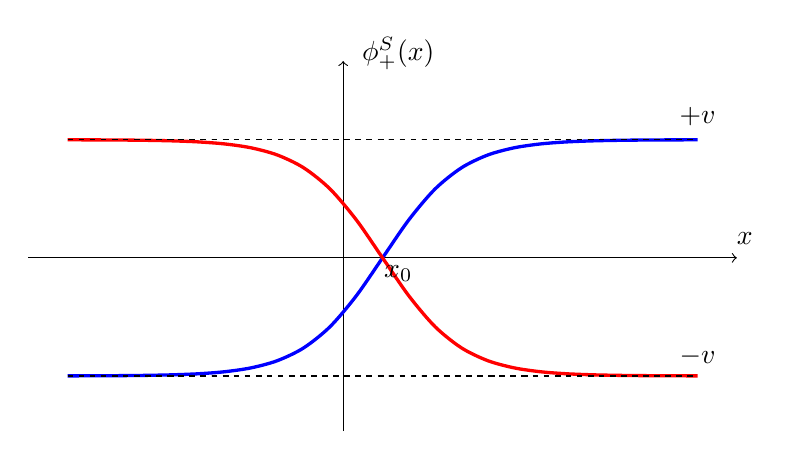
\begin{tikzpicture}
  \draw[->] (-4, 0) -- (5, 0) node[at={(5.1,0.25)}] {$x$};
  \draw[->] (0, -2.2) -- (0, 2.5) node[at={(0.7,2.6)}] {$\phi_+^S(x)$};
  \draw[scale=0.5, domain=-7:9, smooth, variable=\x, blue, very thick] plot ({\x}, {3*tanh(0.5*(\x-1))});
    \draw[scale=0.5, domain=-7:9, smooth, variable=\x, red, very thick] plot ({\x}, {-3*tanh(0.5*(\x-1))});
  \draw[scale=0.5, domain=-7:9, smooth, variable=\x, dash pattern=on 2pt off 2pt] plot ({\x}, {3});
  \draw[scale=0.5, domain=-7:9, smooth, variable=\x, dash pattern=on 2pt off 2pt] plot ({\x}, {-3});
  \draw (4.5,1.8) node {$+v$};
  \draw (4.5,-1.25) node {$-v$};
  \draw (0.7,-0.2) node {$x_0$};
\end{tikzpicture}
\caption{Shape of the solutions $\phi_+^S(x)$ (blue) and $\phi_-^S(x)$ (red).} %parameters: x_0=1, v=3, g=1/3sqrt2 
\label{fig:kink-solution}
\end{figure}

We see that $\phi_+^S$, $\phi_-^S$, $\phi_+^0$ and $\phi_-^0$ cannot be deformed one into other by operations physically implementable, since the boundary conditions at $\infty$ are disjoint. This statement can be translated for the solitons in the conservation of a charge
\begin{eq}\label{eq:cons-charge-kink}
	Q=\int\de x\der{}{x}\phi=\phi(+\infty)-\phi(-\infty)
\end{eq}
which is topological (only the behaviour at infinity is relevant). The corresponding conserved current is 
\begin{eq}
	J_\mu(x)=\lctens_{\mu\nu}\partial^\nu\phi
\end{eq}
with $\mu,\nu=0,1$ where $\mu=0$ is the time $t$ component and $\mu=1$ is the spatial $x$ component, moreover $\lctens$ is the Levi-Civita tensor. We can easily see that $J_0$ actually coincides with the conserved density associated to \eqref{eq:cons-charge-kink}:
\begin{eq}
	\int\de x\, J_0=\int\de x \,\lctens_{0\nu}\partial^\nu\phi=
	\int\de x \,\partial^1\phi=\int\de x\,\pder{}x\phi=Q
\end{eq}
while $J_1$ is the unique component of the vector current. The current $J_\mu$ is automatically conserved without using the equations of motion, since the conservation directly follows from the contraction of a symmetric tensor with an antisymmetric one
\begin{eq}
	\partial^\mu J_\mu=\lctens_{\mu\nu}\partial^\mu\partial^\nu\phi=\lctens_{[\mu\nu]}\partial^{\{\mu}\partial^{\nu\}}\phi=0
\end{eq}

%%%%%%%%%%%%%%%%%%%%%%%
%%%%%%%% LECTURE 12 %%%%%%%%
%%%%%%%%%%%%%%%%%%%%%%%

\subsubsection{The Bogomol'nyi bound}

There is a more instructive way to prove that $\phi_\pm^S$ are the local minima at $(\mp v,\pm v)$ boundary conditions. Let's write the potential $V(\phi)$ in terms of a function $\suppot(\phi)$ called \emph{superpotential} (since it is largely used in supersymmetric theories) by
\begin{eq}
	V(\phi)=\half\left(\der\suppot\phi\right)^2
\end{eq}
Since $V(\phi)=\frac{g^2}4(\phi^2-v^2)^2$ this implies that
\begin{eq}
	\der\suppot\phi=\frac g{\sqrt2}(\phi^2-v^2)
	\tand
	\suppot=\frac g{\sqrt2}\left(\frac13\phi^3-v^2\phi\right)
\end{eq}
The Hamiltonian can be rewritten for $\pi=0$ as
\begin{eq}\label{eq:Ham-kink-suppot}
	H=\int\de x\,\left[\half\left(\der\phi x\pm\der\suppot\phi\right)^2\mp\der\phi x\der\suppot\phi\right]
	\quad\text{for boundary conditions }(\mp v,\pm v)
\end{eq}
Now notice that the last term gives
\begin{eq}
	&\int\de x\,\der\suppot\phi\der\phi x=\suppot(\phi(+\infty))-\suppot(\phi(-\infty)
	=\pm\Delta\suppot\quad\text{for boundary conditions }(\mp v,\pm v)
\end{eq}
with
\begin{eq}
	\Delta\suppot=\suppot(v)-\suppot(-v)=-\frac4{3\sqrt2}gv^3<0
\end{eq}
hence we get that
\begin{eq}\label{eq:Bogom-bound}
	H\geq-\Delta\suppot>0
\end{eq}
for both the possible boundary conditions. This lower bound  is called \emph{Bogomol'nyi bound} (as we will see has several generalizations). This bound is saturated, hence the equality in eq.~\eqref{eq:Bogom-bound} holds, only if the term inside square brackets in eq.~\eqref{eq:Ham-kink-suppot} vanishes, i.e. if the following first order equation is satisfied
\begin{eq}\label{eq:Bogom-bound-cond}
	\der\phi x=\pm\der\suppot\phi
\end{eq}
which coincides exactly with eq.~\eqref{eq:eom-kink}. Hence the solutions $\phi_\pm^S$ are local minima for which the energy coincides with the Bogomol'nyi bound. 

\skipline

The energy density associated to $\phi_\pm^S(x_0)$, depending on the modulus $x_0$, is given by the Hamiltonian density evaluated for the field $\phi_\pm^S(x_0)$ (it obviously depends on the spatial coordinate $x$ and on the choice of $x_0$):
\begin{eq}\label{eq:kink-classic-energy-density}
	\cenergy^\tcl&=\half\left(\der{\phi_\pm^S}x\right)^2+\frac{g^2}4\left(\phi_\pm^{S\,2}-v^2\right)^2
	\overset{\eqref{eq:Bogom-bound-cond}}=2\cdot\half\left(\der{\phi_\pm^S}x\right)^2=\left(\der{\phi_\pm^S}x\right)^2
\end{eq}
In fig.~\ref{fig:kink-energy} one can see the shape of $\cenergy(x)$ associated to the field of fig.~\ref{fig:kink-solution}. It is clearly localized near $x_0$. Hence the soliton exhibits an energy density profile as a `` dump'' around $x_0$, thus behaving ``like a particle'' localized around $x_0$. The integral 
\begin{eq}\label{eq:mass-classical-kink}
	M_S^\tcl:=\int\de x\,\cenergy^\tcl(x)=-\Delta\suppot=\frac4{3\sqrt2}gv^3
\end{eq}
can be interpreted as the ``classical'' mass of the soliton, i.e. the energy of the soliton in its rest frame. 

\begin{figure}[h]
\centering
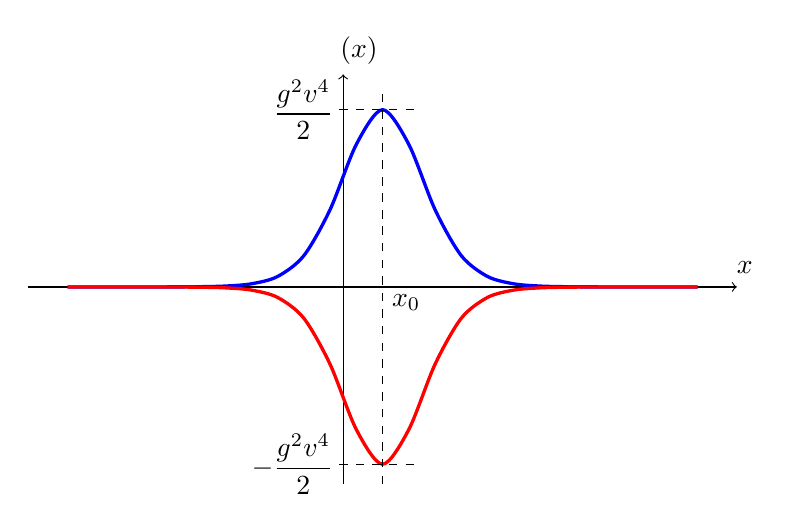
\begin{tikzpicture}
  \draw[->] (-4, 0) -- (5, 0) node[at={(5.1,0.25)}] {$x$};
  \draw[->] (0, -2.5) -- (0, 2.7) node[at={(0.2,3)}] {$\cenergy(x)$};
  \draw[scale=0.5, domain=-7:9, smooth, variable=\x, blue, very thick] plot ({\x}, {4.5*(cosh((\x-1)/2))^(-4)});
  \draw[scale=0.5, domain=-7:9, smooth, variable=\x, red, very thick] plot ({\x}, {-4.5*(cosh((\x-1)/2))^(-4)});
   \draw[scale=0.5, domain=-5:5, smooth, variable=\y, dash pattern=on 3pt off 3pt] plot ({1}, {\y});
   \draw[scale=0.5, domain=-0.1:2, smooth, variable=\x, dash pattern=on 3pt off 3pt] plot ({\x}, {4.5});
   \draw[scale=0.5, domain=-0.1:2, smooth, variable=\x, dash pattern=on 3pt off 3pt] plot ({\x}, {-4.5});
  \draw (0.8,-0.2) node {$x_0$};
  \draw (0,2.25) node [anchor=east]{$\displaystyle\frac{g^2v^4}2$};
  \draw (0,-2.25) node [anchor=east]{$\displaystyle-\frac{g^2v^4}2$};
\end{tikzpicture}
\caption{Shape of the energy density for the fields $\phi_+^S(x)$ (blue) and}{$\phi_-^S(x)$ (red) plotted in fig.~\ref{fig:kink-solution} (the $x$-axis has not been rescaled).} %parameters: x_0=1, v=3, g=1/3sqrt2 
\label{fig:kink-energy}
\end{figure}

Since (looking at the Hamiltonian) the theory is Lorentz invariant (on 1+1 dimension) one can ``change the reference frame'' and make the soliton move at a constant velocity $\textrm v$:
\begin{eq}
	\phi_\pm^S(x,x_0,\textrm v)=\pm v\tanh\left(\frac{gv}{\sqrt2}\,\frac{x-x_0-\textrm vt}{\sqrt{1-\textrm v^2}}\right)
\end{eq}
i.e. behaves like a particle with equation of motion $x=x_0+\textrm vt$.

\subsection{Semi-classical treatment}

Up to now we just described the soliton at classical level. Let us turn to the quantum world. We first give a standard semi-classical (heuristic) Hamiltonian treatment, then we make some comments on a rigorous approach in the spirit of the reconstruction theorem previously discussed. 

\subsubsection{Semi-classical description of fluctuations around the vacuum}

Let us start from the quantization of fluctuations around one vacuum. To quantize perturbatively fluctuations around $\phi_+^0=v$ we rewrite the quantum field as
\begin{eq}
	\ophi(x)=v+\ochi(x)
\end{eq}
Formally (in principle regularizations are needed) expanding in $\ochi$ in the Hamiltonian we get
\begin{eq}	
	H&=\int\de x\,\left[\frac12\opi^2+\frac12\left(\der\ochi x\right)^2+\frac{g^2}4\left(2v\ochi+\ochi^2\right)^2\right]\\
	&=\int\de x\,\left[\frac12\opi+\frac12\left(\der\ochi x\right)^2+\frac{2(gv)^2}2\ochi^2+\polyn(\ochi)\right]
\end{eq}
where $\polyn(\ochi)$ is a polynomial in $\ochi$ of order higher than 2. Integrating by part we get
\begin{eq}
	H_2=\int\de x\,\left[\frac12\opi+\frac12\ochi\left(-\der{^2}{x^2}+2(gv)^2\right)\ochi\right]
\end{eq}
($H_2$ denotes the quadratic part on $H$, describing the free field). One can then expand $\ochi$ in terms of the complete set of solutions of the differential equation
\begin{eq}
	\left(-\der{^2}{x^2}+2(gv)^2\right)\chi_k=\omega^2(k)\chi_k
\end{eq}
which we know are just the complex exponentials $e^{ikx}$ with eigenvalues
\begin{eq}
	\omega^2(k)=k^2+2(gv)^2
\end{eq}
and then one can write
\begin{eq}
	\ochi(x)=\sum_k\op a(k)\chi_k(x)
\end{eq}
From the quadratic terms we see that $\ochi$ is a massive field with (bare) mass $m=\sqrt2gv$, such that we recover the usual dispersion relation $\omega(k)=\sqrt{k^2+m^2}$, and polynomial interaction given by $\polyn(\ochi)$.

Perturbatively we impose the CCR on $\ochi$ and $\opi=\dot\ochi$
\begin{eq}
	[\ochi(x),\opi(y)]=[\ochi(x),\dot\ochi(y)]=i\hbar\,\delta(x-y)
\end{eq}
and in order to make sense to the previous discussion we insert a normal ordering in the Hamiltonian, so that the free $H_2$ Hamiltonian has zero vacuum energy (otherwise it would be divergent) and then proceed in the usual way. 

Clearly in perturbation theory the bare mass of $\ochi$ is renormalized by the polynomial interaction, and the relevant term, coming from $\nord{\ochi^4\!}$, is the counterterm corresponding to the following Feynman graph

\begin{eq}\label{eq:correct-mass-kink-vacuum}
	(-1)\cdot\quad\begin{tikzpicture}[baseline=($(a)+(-90:0.1)$)]	
		\coordinate (a) at (-1.6,0);
		\coordinate (b) at (0,0);
		\coordinate (c) at (1.6,0);	
		\draw (a) -- (c);
		\draw ($(b)+(90:0.6)$) circle(0.6);
		\draw ($(b)+(-90:0.4)$) node {$\displaystyle{g^2}/4$};
		\filldraw [black] (b) circle (2pt);
		\draw ($(a)+(90:0.3)$) node {$\chi$};
		\draw ($(c)+(90:0.3)$) node {$\chi$};
		\draw ($(b)+(90:1.5)$) node {$\chi$};
	\end{tikzpicture}
	\quad=\quad-4\cdot3\cdot\frac{g^2}4\int\frac{\de^2p}{(2\pi)^2}\frac\hbar{p^2+m^2}
	=-\frac{3g^2}{4\pi}\int_0^\infty\de p\der{}{p}\log(p^2+m^2)
\end{eq}
where $4\cdot 3$ is a combinatorial factor\footnote{Notice that the coupling $\frac {g^2}4$ already contains the factor $1/4!$ associated to the possible permutations of the legs of the vertex. This can be easily understood by comparing the interaction potential of the theory with the potential of $\lambda\phi^4$ theory. Since there is only one vertex in the graph no symmetry factor associated to the exchange of the vertices is needed. Hence we just have to take care of the $4\cdot3$ possible ways to connect the external fields to the vertex.}, and we set $\hbar=1$. Introducing a cutoff $\Lambda\gg m$ we get renormalized mass
\begin{eq}\label{eq:classical-mass-kink}
	m^2_R=m^2-\frac{3g^2}{2\pi}\log(\frac{\Lambda^2}{m^2})
\end{eq}
where we multiplied the correction coming from \eqref{eq:correct-mass-kink-vacuum} by 2 in order to take into account the factor 1/2 in the mass term of the Hamiltonian. The quantity $m^2_R$ is exactly the square of the mass that one detects if perform an experimental measure of the mass of the fluctuation $\chi$ around the vacuum. 

\subsubsection{Semi-classical description of fluctuations around soliton solution}

Let us now turn to the quantization around the soliton solution, consider for instance $\phi_+^S$. Since this is a local minima, we can still expand around such solution very similarly to what we done for the fluctuations around the vacuum. First notice that, expressed in terms of the bare mass $m=\sqrt2gv$, the classical mass of the kink eq.~\eqref{eq:mass-classical-kink} reads
\begin{eq}
	M^\tcl_S=\frac {m^3}{3g^2}\sim\frac1{g^2}
\end{eq}
hence it cannot be recovered by a perturbation theory around $g=0$, the perturbative expansion in $g^{-2}$ is not well defined for $g\approx0$. The behaviour $\sim g^{-2}$ of the energy or the action is typical to the soliton solutions. 

A naive approach to quantization would be to write
\begin{eq}
	\ophi(x,t)=\phi_+^S(x)+\ochi(x,t)
\end{eq}
Inserting in the Hamiltonian we get
\begin{eq}
	H &= \int\de x\bigg[\,\half{{\dot\phi^S_+}\hspace{0cm}}^2+\dot\phi^S_+\dot\ochi+\half\dot\ochi^2+\half\left(\der{{\phi_+^S}}x\right)^2+\der{{\phi_+^S}}x\der\ochi x+\half\left(\der\ochi x\right)^2+\\
	&\qquad+\frac{g^2}4\left[({\phi_+^S}^2-v^2)^2+(4{\phi_+^S}^3-4v^2{\phi_+^S})\ochi+(6{\phi_+^S}^2-2v^2)\ochi^2+4{\phi_+^S}\ochi^3+\ochi^4\right]\bigg]
\end{eq}
By integrating by parts with boundary conditions $\ochi(\pm\infty)=0$ (otherwise the field would have infinite energy) we get
\begin{eq}
	H&= \int\de x\bigg[\,\half{{\dot\phi^S_+}{}}^2+\dot\phi^S_+\dot\ochi+\half\dot\ochi^2+\half\left(\der{{\phi_+^S}}x\right)^2-\der{^2\phi_+^S}{x^2}\,\ochi-\half\ochi\,\der{^2\ochi}{x^2}+\\
	&\qquad+\frac{g^2}4\left[({\phi_+^S}^2-v^2)^2+(4{\phi_+^S}^3-4v^2{\phi_+^S})\ochi+(6{\phi_+^S}^2-2v^2)\ochi^2+4{\phi_+^S}\ochi^3+\ochi^4\right]\bigg]
\end{eq}
first notice that the terms linear in $\ochi$ vanish due to the equation of motion of $\phi_+^S$:
\begin{eq}
	\left(\der{^2\phi_+^S}{x^2}-{g^2}({\phi_+^S}^3-v^2\phi_+^S)\right)\ochi=0
\end{eq}
and combining with \eqref{eq:kink-classic-energy-density} we get
\begin{eq}\label{eq:full_ham_fluc}
	H&= M_S^\tcl+\int\de x\bigg[\,\half{{\dot\phi^S_+}\hspace{0cm}}^2+\dot\phi^S_+\dot\ochi+\half\dot\ochi^2-\half\ochi\,\der{^2\ochi}{x^2}+\frac{g^2}4\left[(6{\phi_+^S}^2-2v^2)\ochi^2+4{\phi_+^S}\ochi^3+\ochi^4\right]\bigg]\\
	&=M_S^\tcl+\int\de x\bigg[\,\half{{\dot\phi^S_+}\hspace{0cm}}^2+\dot\phi^S_+\dot\ochi+\half\dot\ochi^2+\half\ochi L_2\ochi+\frac{g^2}4\left(4{\phi_+^S}\ochi^3+\ochi^4\right)\bigg]
\end{eq}	
with
\begin{eq}
	L_2=\frac{g^2}2(6{\phi_+^S}^2-2v^2)-\der{^2}{x^2}=\frac{m^2}{2}\left(3\tanh^2\frac{mx}2-1\right)-\der{^2}{x^2}
\end{eq}
Up to now we kept terms proportional to $\dot\phi^S_+$ because in the following we will introduce a time dependence in $\phi^S_+$, nevertheless at this stage the field is constant, hence taking the terms quadratic in $\ochi$ we get
\begin{eq}\label{eq:kink-H_2-fluct}
	H_2=\int\de x\,\left(\half\dot\ochi^2+\frac12\ochi L_2\ochi\right)
\end{eq}
and the remaining terms are third and quartic interactions in $\ochi$.

Now the problem is similar to the free one, except for the fact that the operator associated to the harmonic oscillator has been replaced by $L_2$. We have to solve the ``Schrödinger equation''
\begin{eq}
	L_2\chi_n(x)=\omega_n^2\chi_n(x)
\end{eq}
where $n$ and $\chi_n$ play the previous roles of $k$  and $e^{ikx}$ respectively. Then we can rewrite
\todo{A lezione lei aveva preso $n\in\N$. Assumendo invece $n\in\Z$ otteniamo il fattore 2 necessario a rendere esatto il risultato a fine sezione, di cui le parlavo quando ci siamo sentiti.}
\begin{eq}
	\ochi(x,t)=\sum_{n\in\Z}\op a_n(t)\chi_n(x)
\end{eq}
We can rewrite the Hamiltonian as
\begin{eq}
	H_2=\sum_{n\in\Z}\frac{\dot{\op a}_n^2}2+\frac{\omega_n^2}2\op a_n^2
\end{eq}
i.e. naively as a sum of uncoupled oscillator, as in the free case. 

\skipline

This would actually be true if $\omega_n>0$, but one can prove that there is one vanishing eigenvalue $\omega_0$, it is a ``zero mode'' and must be treated separately because the fluctuations along the direction of this mode are not small.\footnote{Fluctuations associated to $\omega_n=0$ are not limited by any physical argument, as the kinetic energy is identically vanishing for this mode. Even worse, $\omega_n<0$ would imply that the system is unstable, as fluctuations naturally become arbitrarily large. Luckily, the last case does not occur in our treatment.} Such zero mode is associated to fluctuations of the modulus of kink solution: changing the value of $x_0$ the solution has the same energy as the original one, hence this do not contribute to the Hamiltonian, moreover there is no limit of this kind of fluctuations, as all possible values of $x_0$ give  kink solutions with the same energy. 

The occurrence of the zero mode can be understood by a general argument. The kink solution depend on the fixed value $x_0$, hence fixing the solution the translational invariance has been explicitly broken in the space of equilibrium states.\footnote{This is very similar to the previous example of a classical particle in a flat plane, subject to a gravitational force.} Such invariance is recovered by taking into account all possible values of $x_0$, and the standard approach, called \emph{adiabatic}, to recover the invariance is to convert the position $x_0$ of the soliton into a quantum dynamical variable $\op x_0(t)$ (a quantum position variable cannot assume a sharp value, hence there is no breaking of translational invariance) and to assume that the only dependence on time of the kink solution enter trough its modulus\footnote{Adiabaticity means ``very slow changes'' of the system, in this way translations of the modulus are slow enough to leave invariant the shape of the field during the variation of $x_0$. This motivates the dependence on time of the kink only through $x_0(t)$.}
\begin{eq}\label{eq:adiabatic-solution-kink}
	\phi_+^S(x)\longmapsto \phi_+^S(x-\op x_0(t))
	\tand
	\chi_n(x)\longmapsto\chi_n(x-\op x_0(t))
\end{eq}
Notice this is in agreement with the previous interpretation of the classical kink as a localized particle, indeed moving to a quantum mechanical description a semi-classical\footnote{I.e. without any other quantum number.} particle should only depend on a quantum operator describing its position. 

Expanding $\ophi$ in $\op x_0$ we are able to recover the quantum mechanics of the kink. The same adiabatic strategy apply in general for the description of the solitons, but we will discuss it in details only in this instance. For example the time derivative of $\ophi$ is given by (notice that using the adiabatic approach we eliminated the zero mode $\omega_0$)\footnote{Let $\Z^*:=\Z\setminus\{0\}$ be the set of non-zero integers.}
\begin{eq}\label{eq:kink-time-der-adiab}
	\dot\ophi(x,t)
	&=\der{}{t}\left(\phi_+^S(x-\op x_0(t))+\ochi(x-\op x_0(t),t)\right)
	=\der{}{t}\left(\phi_+^S(x-\op x_0(t))+\sum_{n\in\Z^*}\op a_n(t)\chi_n(x-\op x_0(t))\right)\\
	&=\left[-\der{\phi_+^S(x-\op x_0(t))}x-\sum_{n\in\Z^*}\op a_n(t)\der{\chi_n(x-\op x_0(t))}x\right]\dot{\op x}_0(t)+\sum_{n\in\Z^*}\dot{\op a}_n(t)\chi_n(x-\op x_0(t))\\
	&=\left[-\der{\phi_+^S(x-\op x_0(t))}x-\der{\ochi(x-\op x_0(t),t)}x\right]\dot{\op x}_0(t)+\sum_{n\in\Z^*}\dot{\op a}_n(t)\chi_n(x-\op x_0(t))\\
	&=-\der{\ophi(x,t)}x\dot{\op x}_0(t)+\sum_{n\in\Z^*}\dot{\op a}_n(t)\chi_n(x-\op x_0(t))
\end{eq}
Notice that the second term in the square bracket, when multiplied with $\dot{\op x}_0(t)$, give a product of operators and in general it gives a negligible contribution respect to the other terms.\footnote{A better motivation of this claim will be given in the following.} 
The Hamiltonian around the soliton up to quadratic terms is
\begin{eq}
	H_{\leq2} &\smash{\overset{\eqref{eq:full_ham_fluc}}=}M_S^\tcl+\int\de x\bigg[\,\half{{\dot\phi^S_+}\hspace{0cm}}^2+\dot\phi^S_+\dot\ochi+\half\dot\ochi^2+\half\ochi L_2\ochi\bigg]\\
	&\smash{\overset{\eqref{eq:kink-time-der-adiab}}=}M_S^\tcl+\int\de x\,\bigg[\,\left(\der{\phi_+^S}x\right)^2\dot{\op x}\hspace{0cm}^2_0-\der{\phi_+^S}x\dot{\op x}_0\dot\ochi+\half\dot\ochi^2+\half\ochi L_2\ochi\bigg]
\end{eq}
As a consequence of the adiabaticity assumption\footnote{From the practical point of view, this consist in assuming that our ``particle'' moves very slowly, in such a way that the motion do not affect the shape of the field.} the effect of the time dependence of the modulus and the presence of the fluctuations should be considered separately in the Hamiltonian, i.e. the term $\dot{\op x}_0\dot\ochi$ gives higher order corrections which we can neglect. From another point of view, typically the Fourier transform of $\dot{\op x}_0$ should have low frequencies components, whereas typically fluctuations highly oscillate, hence the support in the Fourier space of $\op\ochi$ is typically charaterized by high frequencies. Since Fourier components of different wavelengths are orthogonal we get $\int\de x\,\dot{\op x}_0\dot\ochi\approx0$. For the same reason, we neglected $\der\chi x\dot{\op x}_0$ in \eqref{eq:kink-time-der-adiab}. Using eq.~\eqref{eq:kink-classic-energy-density} we finally get
\begin{eq}\label{eq:quadr-ham-quantum-kink}
	H_{\leq2} &=M_S^\tcl+\half M_S^\tcl \,\dot{\op x}\hspace{0cm}^2_0+\int\de x\,\bigg[\half\dot\ochi^2+\half\ochi L_2\ochi\bigg]\\
	&=M_S^\tcl+\half M_S^\tcl \,\dot{\op x}\hspace{0cm}^2_0+\sum_{n\in\Z^*}\frac{\dot{\op a}_n^2}2+\frac{\omega_n^2}2\op a_n^2\\
	&=M_S^\tcl+\frac{\op p_0^2}{2M_S^\tcl}+\sum_{n\in\Z^*}\frac{\dot{\op a}_n^2}2+\frac{\omega_n^2}2\op a_n^2
\end{eq}
where we introduced the momentum $\op p_0:=M_S^\tcl\dot{\op x}_0$. In this expression we have three contribution: the classical mass of the soliton, a term corresponding to the kinetic energy of the soliton as a quantum particle, and a set of oscillators describing the effect of oscillations around the classical solution. Recall that we made an expansion in $\dot {\op x}_0$ in a relativistic framework, hence we can reconstruct the complete energy of the soliton meant as a quantum particle:
\begin{eq}
	 M_S^\tcl+\frac{\op p_0^2}{2M_S^\tcl} \quad\longrightarrow\quad \sqrt{\smash[b]{M_S^\tcl+\op p_0^2}}
\end{eq}
(we won't use the complete energy since we are working at quadratic order in the operators).
Notice that there is no potential for $\op x_0$, because consistently with translational invariance $H$ cannot depend on $\op x_0$ itself but only on $\op p_0$.
Quantization is finally archived imposing commutation relations
\begin{eq}
	[\op x_0,\op p_0]=i
	\tand
	[\op a_n,\dot{\op a}_m]=i\delta_{nm}
\end{eq}

%%%%%%%%%%%%%%%%%%%%%%%
%%%%%%%% LECTURE 13 %%%%%%%%
%%%%%%%%%%%%%%%%%%%%%%%

Using eq.~\eqref{eq:quadr-ham-quantum-kink} one can approximatively compute the renormalization of the mass $M_S^\tcl$ due to the quantum modes. First notice that since non-zero modes are oscillatory modes we know that
\begin{eq}
	\spec\left(\sum_{\in\Z^*}\frac{\dot{\op a}_n^2}2+\frac{\omega_n^2}2\op a_n^2\right)=\sum_{n\in\Z^*}\left(N_n+\half\right)\omega_n
	\twith N_n\in\N \tforall n\in\Z^*
\end{eq}
Hence in its ground state ($N_n=0$, $p_0=0$) the energy of the kink becomes
\begin{eq}
	M_S^\tcl+\sum_{n\in\Z^*}\frac{\omega_n^2}2
\end{eq}
However we should remember that in RQFT the Hamiltonian is defined so that the vacuum (perturbatively) is annihilated by $H$, hence we have to subtract to the previous expression the vacuum expectation value of the ``unrenormalized'' Hamiltonian $H_{\leq2}$. Therefore, the energy of the ground state for the Hamiltonian is 
\begin{eq}\label{eq:kink-quantum-mass-renorm}
 	M_S^\tq=M_S^\tcl+\sum_{n\in\Z^*} \frac{\omega_n}2-\frac{\omega_{\tvac,n}}2
\end{eq}
where $\omega_{\tvac,n}$ are the frequencies of the oscillator modes in the vacuum. In the thermodynamic limit $L\to\infty$ these are labelled by a continuum index $p$ are since we are in a relativistic context the on-shell condition implies $\omega_n\to\omega(p)=\sqrt{p^2+m^2}$. To get a well defined subtraction in $M_S^\tq$ we first put the system in a region of length $L$ finite, and then we take the limit $L\to\infty$. One can fix the boundary conditions in some different ways provided that in the thermodynamic limit they coincide with the previous ones. We use the (Dirichlet) vanishing boundary conditions at the boundary of $L$, such that
\begin{eq}
	\omega_{\tvac,n}=\sqrt{p_n^2+m^2}
	\twith
	p_nL=\pi n
\end{eq}

For $H_2$, apart from the eigenvalue 0, there is an eigenvalue $\omega_1=\frac{\sqrt3}2m$ while all the other eigenvalues lie above $m^2$. In the thermodynamic limit the eigenvalues larger than $m^2$ are still given by a continuum $\omega(\tilde p)=\sqrt{\smash{\tilde p}^2+m^2}$ corresponding to the asymptotic behaviour of the eigenfunctions of the operator $L_2$
\begin{eq}	
	\chi_{\tilde p}(x)&\xrightarrow[x\to+\infty]{}e^{\pm i\tilde p x}\\
	&\xrightarrow[x\to-\infty]{}e^{\pm i(\tilde px+\delta(\tilde p))}
\end{eq}
where $e^{i\delta(\tilde p)}$ is a correction called \emph{phase shift} (as it gives an phase shift to the asymptotic behaviour) which always comes out for non-trivial scatterings and is given by
\begin{eq}\label{eq:kink-phase-shift}
	e^{i\delta(\tilde p)}=e^{ i\big[2\arctan\frac{\tilde p}m+2\arctan\frac{2\tilde p}m\big]}
\end{eq}
For the system at finite length with 0-boundary conditions the phase shift is given by
\begin{eq}
	\tilde p_nL-\delta(\tilde p_n)=\pi n=p_nL
	\tfor
	n\in\N
\end{eq}
Then eq.~\eqref{eq:kink-quantum-mass-renorm} reads (discarding the finite difference due to the eigenvalue $\omega_0$ and $\omega_1$, as we are interested in the divergent terms)
\begin{eq}
	 M_S^\tq-M_S^\tcl&\approx\sum_{n\in\Z^*}\left(\frac{\sqrt{\tilde p^2_n+m^2}}2-\frac{\sqrt{p^2_n+m^2}}2\right)
\end{eq}
Going to the thermodynamic limit and using $n=p_nL/\pi=(\tilde p_nL-\delta(\tilde p_n))/\pi$ we can replace\footnote{The value $p=0$ has zero measure, hence we can include it in the integral.}
\begin{eq}
	\sum_{n\in\Z^*}\quad\longmapsto\quad\int_{-\infty}^\infty\frac{\de p\,L}\pi
\end{eq}
and then we get
\begin{eq}
	 M_S^\tq-M_S^\tcl&\approx\half\int_{-\infty}^\infty\frac{\de p\,L}\pi\left(\sqrt{\left(p+\frac{\delta(p)}L\right)^2+m^2}-\sqrt{p^2+m^2}\right)
	\smash{\overset{\delta(p)\ll L}\approx}\ \int_{-\infty}^\infty\frac{\de p}{2\pi}\,\frac{p\,\delta(p)}{\sqrt{p^2+m^2}}\\
	&=\int_{-\infty}^\infty\frac{\de p}{2\pi}\,\delta (p)\,\der{\sqrt{p^2+m^2}}p
	=\int_0^\infty\frac{\de p}{\pi}\,\delta (p)\,\der{\sqrt{p^2+m^2}}p
\end{eq}
where in the third step we expanded around $\delta(p)/L\approx 0$ and in the last we used $\delta(p)=-\delta(-p)$.
Integrating by parts with boundary conditions $\delta(0)=\delta(\infty)=0$ (directly follows from eq.~\eqref{eq:kink-phase-shift}) we finally get
\begin{eq}
	 M_S^\tq-M_S^\tcl&=-\int_0^\infty\frac{\de p}{\pi}\sqrt{p^2+m^2}\,\der{\delta(p)}p
	\smash{\overset{\eqref{eq:kink-phase-shift}}=}-\int_0^\infty\frac{\de p}{\pi}\sqrt{p^2+m^2}\left(\frac{2m}{p^2+m^2}+\frac{4m}{4p^2+m^2}\right)\\
	&=-\frac{2m}{\pi}\int_0^\infty\de y\,\sqrt{y^2+1}\left(\frac1{y^2+1}+\frac2{4y^2+1}\right)
	\quad\twith y=\frac pm
\end{eq}
The last integral is clearly logarithmically divergent. Introducing a cutoff $\Lambda$ the divergent term is indeed (the previous integral is well defined for small $p$, hence we consider only the high energy part)
\begin{eq}\label{eq:kink-div-bare-mass}
	 M_S^\tq-M_S^\tcl\approx-\frac{3m}{\pi}\int^{\Lambda/m}\frac{\de y}{y}=-\frac{3m}{\pi}\log\frac\Lambda m=-\frac{3m}{2\pi}\log\frac{\Lambda^2}{m^2}
\end{eq}
This divergence turns out since we considered the unrenormalized mass rather than the renormalized one, indeed in our discussion so far we did not take into account higher order interactions. We should take into account divergences due to third and quartic coupling, as we have done for the fluctuations around the vacuum.

Using the result eq.~\eqref{eq:classical-mass-kink} for $\delta m^2$, this correction on the mass implies a corresponding correction to the energy density:
\todo{Non capisco come si ottenga la seguente formula. Mi sembrerebbe più naturale usare $\half\delta m(\phi_{\text{kink}}^2-\phi_{\text{vac}}^2)$}
\begin{eq}
	\delta\cenergy=-\half\delta m^2(\phi_{\text{kink}}^2-\phi_{\text{vac}}^2)=\half\delta m^2v^2\left(1-\tanh^2\frac{gv(x-x_0)}{\sqrt2}\right)
\end{eq}
which, by integration, give the mass one-loop correction
\begin{eq}
	\delta M&=\half\delta m^2\frac{m^2}{2g^2}\int_{-\infty}^{+\infty}\de x\,\left(1-\tanh^2\frac m2(x-x_0)\right)\\
	&=\delta m^2\,\frac{m}{2g^2}\int_{-\infty}^{+\infty}\de y\,\der{}y\tanh y	\quad\twith y=\half m(x-x_0)\\
	&=\delta m^2\,\frac{m}{g^2}\ 
	\smash{\overset{\eqref{eq:classical-mass-kink}}=}\, -\frac{3m}{2\pi}\log\frac{\Lambda^2}{m^2}
\end{eq}
\todo{Penso che il segno $-$ in $\delta\cenergy$ sia sbagliato, togliendolo il risultato cancella \eqref{eq:kink-div-bare-mass} visto che hanno segni opposti. }
which is exactly the factor needed to cancel the divergence in the bare mass of $\chi$ in eq.~\eqref{eq:kink-div-bare-mass}. So the counterterm needed for the $\chi$ mass renormalization makes finite also the quantum correction (perturbatively) to the kink mass. 

\subsection{Applications}

Before leaving the semi-classical treatment of the kink let us comment some physical applications. 

\subsubsection{High-energy physics}

Let's consider the same theory in $D=3+1$ dimension. Then adding two dimensions, the ``soliton'' center $x_0$ instead of a point become a plane (along $y$ and $z$ directions), and the kink become a \emph{domain wall}, as it separates the space in two domains. Clearly in the thermodynamic limit the energy of such object is infinite, but the energy per unit area $A$
\begin{eq}
	T=\frac HA
\end{eq}
is still finite and is called \emph{wall tension}. Notice that the energy $H$ is not well defined as it is divergent, but still we can define $T$ and then take its thermodynamic limit, which is well-defined. The world with a domain wall is disjoint from the world without a domain wall, hence we have a spontaneous breaking of translational invariance, except for some special instances, for example in the case of space-time with a particular topology (e.g. if the space-time is a torus, then $H$ and $A$ are finite and the wall just ``open'' the torus in a cylinder) or in the case where the wall is a purely quantum effect and has a ``virtual area'', i.e. it exists only for finite time. 

In $D>2$ the quantum version of $x_0$, $\op x_0(t)$, becomes a function of the coordinate of the wall,  for example in $D=4$ we have $\op x_0(t,y,z)$. A calculation completely analogous to the previous one gives the following Hamiltonian (at quadratic order) for the kink
\begin{eq}
	H_{\leq 2}=\int\de t\,\de y\,\de z\,\half\left[\op p_0(t,y,z)^2+\left(\partial_y{\op x_0}(t,y,z)\right)^2+\left(\partial_z{\op x_0}(t,y,z)\right)^2\right]
\end{eq}
A complete treatment including higher order terms in the Lagrangian formalism give the so called \emph{Nambu-Goto} or \emph{Polyakov actions}. Moreover, if a domain world is coupled to gravity, it ``antigravitates'', that is, it is repulsive for both other walls or for massive particles. 

\subsubsection{Solid state physics}

Kinks appear in many materials, especially in those which can be described as one-dimensional chains. A famous one is the polyacetylene. This is a linear polymer made of a sequence of units of $(\text C_2\text H_2)_n$ with two minimal energy configurations, shown in fig.~\ref{fig:polyacetylene}, which can be obtained from each other by reflection, i.e. by a $\Z_2$ symmetry.

\setchemfig{atom sep=2.5em}
\begin{figure}[h]
	\centering
	\scalebox{0.9}{
		\chemfig{-[:-30]C(-[:-90]H)=[:30]C(-[:90]H)-[:-30]C(-[:-90]H)=[:30]C(-[:90]H)-[:-30]C(-[:-90]H)=[:30]C(-[:90]H)-[:-30]C(-[:-90]H)=[:30]C(-[:90]H)-[:-30]C(-[:-90]H)=[:30]C(-[:90]H)-[:-30]}
	}
	\quad
	\scalebox{0.9}{
		\chemfig{=[:-30]C(-[:-90]H)-[:30]C(-[:90]H)=[:-30]C(-[:-90]H)-[:30]C(-[:90]H)=[:-30]C(-[:-90]H)-[:30]C(-[:90]H)=[:-30]C(-[:-90]H)-[:30]C(-[:90]H)=[:-30]C(-[:-90]H)-[:30]C(-[:90]H)=[:-30]}
	}
	\caption{Two minimal energy configurations of \emph{trans}-polyacetylene.}
	\label{fig:polyacetylene}
\end{figure}

A kink interpolates between the two structures and in terms of the displacement of the double bond it has exactly the form of the kink of $\phi^4$ in the lattice renormalization. An example of such situation is shown in fig.~\ref{fig:kink-polyacetylene}.

\begin{figure}[h]
	\centering
	\scalebox{0.9}{
		\chemfig{-[:-30]C(-[:-90]H)=[:30]C(-[:90]H)-[:-30]C(-[:-90]H)=[:30]C(-[:90]H)-[:-30]C(-[:-90]H)-[:30]C(-[:90]H)=[:-30]C(-[:-90]H)-[:30]C(-[:90]H)=[:-30]C(-[:-90]H)-[:30]C(-[:90]H)=[:-30]}
	}
	\caption{A state of \emph{trans}-polyacetylene chain with one of the double bonds\\converted into a single bond form a domain wall.}
	\label{fig:kink-polyacetylene}
\end{figure}

There are a lot of one-dimensional systems with $n$ ground states related by $\Z_n$ symmetry, spontaneously broken, which exhibits kinks interpolating between these ground states. 

\subsection{Quantum field theory treatment}

\cite{Marchetti:1986bda}, \cite{Marchetti:1987pz}, \cite{Frohlich:1987er}, \cite{Frohlich:1987gu}, \cite{Frohlich:1990tc}\\

Up to now we have discussed classical and quantum mechanical treatment of kinks. What about a really QFT treatment?

\subsubsection{The space of configurations of the path integral}

We start by asking how much the classical solution of a field theory is relevant for understanding the corresponding QFT behaviour. 
In the path-integral approach the configurations of the field $\phi(x)$ are weighted by $e^{-\frac1\hbar S(\phi)}$, where $S(\phi)$ is the classical action, and the classical equations of motion can be derived as minima of $S(\phi)$. 

The naive answer to the above question is that classical solutions give the dominant contribution to the path integral at least in the semi-classical limit of small $\hbar$ or more in general if the action contribution $e^{-S(\phi)}$ dominates over the measure $\pide\phi$, e.g. when one can rewrite the action in the form $\beta S(\phi)$ with $\beta$ sufficiently large.\footnote{This is often the case for supersymmetric theories, at least in low dimensions.} In our $\phi^4$ model this is achieved rescaling
\begin{eq}
	\phi\to g\phi
\end{eq}
so that
\begin{eq}
	S(\phi)\to\frac1{g^2}\int\dd^2x\,\left(\half\dot\phi^2+\half\left(\der\phi{x}\right)^2+\frac14\left(\phi-(vg)^2\right)^2\right)
\end{eq}
hence for small $g^2$, keeping $vg$ fixed, the exponential weight is dominant in the path integral. 

However, if there is no UV cutoff, this naive reasoning is wrong, because the typical configurations of $\phi$ are extremely singular, whereas solutions of equations of motion are typically very regular. If we consider just the quadratic term of the action, denoted by $Q(\phi)$, there is a simple way to understand the typical regularity of $\phi$. Let formally
\begin{eq}
	C(x-y)\equiv\langle\phi(x)\phi(y)\rangle_2:=\frac{\displaystyle\int\pide\phi\,e^{-Q(\phi)}\phi(x)\phi(y)}{\displaystyle\int\pide\phi\,e^{-Q(\phi)}}
\end{eq}
usually called \emph{covariance}, then assuming translational invariance we can perform the Fourier transform of $C$, $\tilde C(k)$, and then there is a theorem proving that typical configurations of $\phi$ satisfy with probability 1 the estimate
\begin{eq}\label{eq:property-covariance}
	|\phi(x)-\phi(y)|<\text{const}\cdot|x-y|^\alpha
\end{eq}
for every $\alpha$ such that 
\begin{eq}\label{eq:property-covariance-cond}
	\int\de^D k\,\tilde C(k)\,k^{2\alpha}<\infty
\end{eq}
Conversely, eq.~\eqref{eq:property-covariance} is almost never satisfied if eq.~\eqref{eq:property-covariance-cond} does not hold. 

For $D=1$ (i.e. $\phi(x)=q(t)$, we are in the quantum mechanical case) with 
\begin{eq}
	\tilde C(k_0)=\frac1{k_0^2+m^2}
\end{eq}
which is the case for the harmonic oscillator, we have
\begin{eq}
	\int\de k_0\,\frac1{k_0^2+m^2}\,k_0^{2\alpha}<\infty
	\quad\text{only if}\quad
	\alpha<\half
\end{eq}
hence $q(t)$ is continuous in $t$ (continuity is ensured by $\alpha>0$) but it is not differentiable (differentiability requires $\alpha>1$).\footnote{This may be interpreted as follows: since at any time the particle can be found at an arbitrary position, the probability that the sequence of positions follows a smooth path is practically vanishing.}

For arbitrary $D$ and 
\begin{eq}
	\tilde C( k)=\frac1{ k^2+m^2}
\end{eq}
condition eq.~\eqref{eq:property-covariance-cond} is satisfied provided that $D+2\alpha<2$ holds. This means that $\phi(x)$ is not even continuous for $D\geq2$. For this reason our initial claim is wrong, and classical solutions are not the dominant contributions to the path integral. Notice that the situation become worse and worse as we increase $D$, since greater values of $D$ implies smaller values of $\alpha$. The reason behind this is that higher is the dimension, stronger are the ultraviolet effects, as one can easily see this fact from dimensional analysis. 

Typical configurations of $\phi$ are distributions. In a sense we should expect this, since quantum fields are described by operator-valued distributions in the operator formalism. It turns out that configurations with finite action are of measure 0 in the space of all field configurations over which the path integral is performed. 

Summarizing, for a theory where the ultraviolet cutoff is pushed to infinity and the translational invariance holds, we can apply the previous theorem, which tells us exactly what happens when the path integral is Gaussian, i.e. when the action si quadratic, described by $Q$.  In particular, we know that typical configurations are extremely singular: they are mostly continuous only in $D=1$, whereas in all dimensions are not differentiable. As we will see, this suggest which configurations dominate the path integral, and the description of such configuration will lead us to the notion of \emph{defects}, which is the corner stone for the description of solitons in QFT. 

\skipline

%%%%%%%%%%%%%%%%%%%%%%%
%%%%%%%% LECTURE 14 %%%%%%%%
%%%%%%%%%%%%%%%%%%%%%%%




%%%%%%%%%%%%%%%%%%%%%%%
%%%%%%%% LECTURE 15 %%%%%%%%
%%%%%%%%%%%%%%%%%%%%%%%

\end{document}